\section{Graphic adapter}

Graphics adapters partition the screen into a grid of discrete elements known as pixels, each capable of displaying a specific color. 
These pixels collectively render images sampled from spatial data, enabling the adapter to accurately display them on a monitor.
To facilitate this process, the adapter is equipped with dedicated memory known as video memory (VRAM).

\begin{figure}[H]
    \centering
    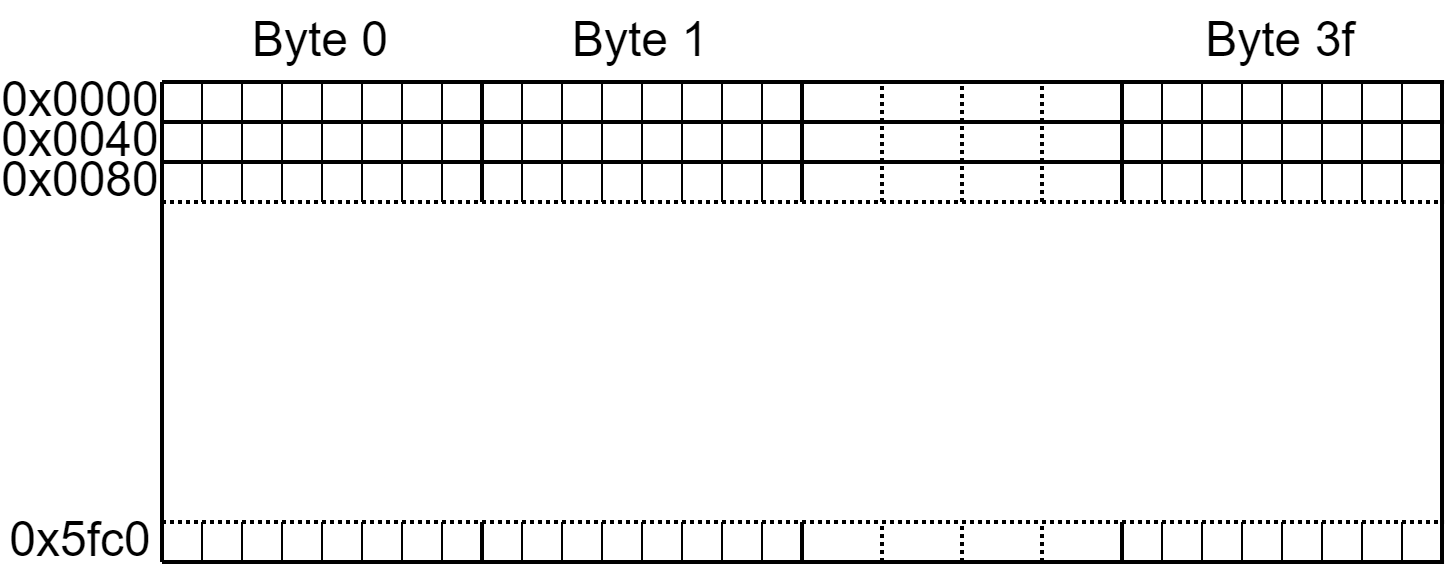
\includegraphics[width=0.5\linewidth]{images/adapter.png}
    \caption{VRAM's structure}
\end{figure}

A segment of the VRAM, referred to as the screen buffer or frame buffer, contains encoded color information for all the pixels displayed on the screen.
A specialized component on the graphics card, such as the RAMDAC for analog displays, utilizes this information from the VRAM to construct the image on the display.
Users typically do not interact directly with the screen buffer; instead, they store images in various sections of the VRAM.\@
Subsequently, users compose the on-screen image by issuing commands to the graphics adapter.
These commands can include drawing points, lines, and other shapes, writing text, transferring raster images from the VRAM, performing 3D projections, and applying deformations and effects to the images. 
By combining these commands with the data stored in the VRAM, the adapter constructs the final image and transmits it to the display.

Performing complex operations involves various tasks such as interacting with multiple displays, managing multiple graphic adapters, or displaying multiple images simultaneously (e.g., stereoscopy), which can introduce significant complexity.

\paragraph*{Vulkan}
Graphics adapters are typically developed in conjunction with their software drivers, ensuring that programmers interface with the hardware through libraries provided by the manufacturer rather than directly accessing video card registers. 
Vulkan exemplifies a platform-independent standard set of procedures that streamlines the access of graphic card functionalities by application code.